% Based on Model 3 in "Activity 13 Encryption" by Helen Hu

\model{Caesar Cipher}

Julius Caesar famously used a ``Cipher Wheel'' to encrypt his messages to Cicero.
This website provides an electronic version of the cipher wheel:

\begin{center}
\url{http://cryptoclub.math.uic.edu/shiftcipher/shiftcipher.htm}
\end{center}

The Cipher Wheel uses a shift of the alphabet to determine which letters should be substituted.
The outer ring is the original characters in \textbf{plaintext} (the first row of characters); the inner ring is the encrypted characters in \textbf{ciphertext} (the second row of characters).

\begin{center}
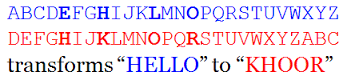
\includegraphics[height=0.65in]{CSP/caesar1.png}
\end{center}


\quest{15 min}


\Q In both the above model and in the electronic cypher wheel, blue (1st line) and red (2nd line) display the same set of characters.
Which color/line represents the original characters, and which color/line represents the encrypted characters?

\begin{answer}[3em]
Red is encrypted (ciphertext), and blue is original (plaintext).
\end{answer}


\Q Rotate the electronic cypher wheel to match the blue and red characters above, by clicking on the green arrows.
What is the key (the shift)?

\begin{answer}[3em]
The key is 3: A shifts to D, three letters to the right.
\end{answer}


\Q Assume we do not know the key, but we know a Caesar encryption was used to encrypt this following ciphertext.
Using trial and error, decrypt the phrase:

\begin{center}
PDA XAOP PDEJCO EJ HEBA WNA BNAA
\end{center}

\begin{enumerate}

\item What is the original text?
\ans{THE BEST THINGS IN LIFE ARE FREE}

\item What is the key (the shift)?
\ans{The key is 22: A shifts to W, three letters to the left.}

\end{enumerate}


\Q Consider how we might decrypt the phrase without the key.

\begin{enumerate}

\item How many different keys are there?

\ans{There are 26 keys; however, the key of zero is worthless.}

\item Describe the process that YOU used to decrypt a phrase when the key was unknown.

\begin{answer}
We guessed the first word might be THE, and then we lined up the wheel on cryptoclub to decrypt the rest.
\end{answer}

\item In contrast, describe the process a COMPUTER could use to decrypt a phrase when the key is unknown.

\begin{answer}
Computers can simply try all 26 keys, one by one.
They can also use a spell checker to see if the answer contains English words.
\end{answer}

\end{enumerate}


\Q Think about the examples you brainstormed at the beginning of the activity.
What is one advantage and one disadvantage of using Caesar Cipher encryption for online security?

\begin{enumerate}

\item one advantage: \ans{It's very simple and fast to compute.}

\item one disadvantage: \ans{It's very easy to guess the key.}

\end{enumerate}
